% XeLaTeX can use any Mac OS X font. See the setromanfont command below.
% Input to XeLaTeX is full Unicode, so Unicode characters can be typed directly into the source.

% The next lines tell TeXShop to typeset with xelatex, and to open and save the source with Unicode encoding.

%!TEX TS-program = xelatex
%!TEX encoding = UTF-8 Unicode

\documentclass[12pt,titlepage]{article}
\usepackage{geometry}
 \geometry{
 a4paper,
 left=25mm,
 right=25mm,
 top=25mm,
 bottom=25mm
 } 
%\geometry{landscape}                % Activate for for rotated page geometry
%\usepackage[parfill]{parskip}    % Activate to begin paragraphs with an empty line rather than an indent
\usepackage{graphicx}
\usepackage{amssymb}
\usepackage{amsmath}
\usepackage{float}
\usepackage{siunitx}
\usepackage{booktabs}
\usepackage[textfont={it}]{caption}
\usepackage{subcaption}
\usepackage[htt]{hyphenat}
\usepackage[]{algorithm2e}
\SetAlCapNameFnt{\it} 
\SetAlCapFnt{\rm}
\graphicspath{{../notebooks/pics/}}
% Will Robertson's fontspec.sty can be used to simplify font choices.
% To experiment, open /Applications/Font Book to examine the fonts provided on Mac OS X,
% and change "Hoefler Text" to any of these choices.

\def\labelitemi{--}

\usepackage{fontspec,xltxtra,xunicode}
\defaultfontfeatures{Mapping=tex-text}
\setromanfont[Mapping=tex-text]{Palatino}
\setsansfont[Scale=MatchLowercase,Mapping=tex-text]{Gill Sans}
\setmonofont[Scale=MatchLowercase]{Andale Mono}
\setlength\parindent{0pt}

\title{\vspace{-4em}\noindent\rule{\textwidth}{.5pt}\\\emph{Predicting Terror Attacks?}\\A Data Story\\
\vspace{-.6em}\noindent\rule{\textwidth}{.5pt}}
\author{Axel Nilsson, Nicolas Bollier, Elias Le Boudec, Enea Figini\\Team 29}
%\date{}                                           % Activate to display a given date or no date
\makeatletter
\renewcommand{\@algocf@capt@plain}{above}% formerly {bottom}
\makeatother

\begin{document}
\maketitle
\pagebreak
% For many users, the previous commands will be enough.
% If you want to directly input Unicode, add an Input Menu or Keyboard to the menu bar 
% using the International Panel in System Preferences.
% Unicode must be typeset using a font containing the appropriate characters.
% Remove the comment signs below for examples.

% \newfontfamily{\A}{Geeza Pro}
% \newfontfamily{\H}[Scale=0.9]{Lucida Grande}
% \newfontfamily{\J}[Scale=0.85]{Osaka}

\section{Introduction}
\label{sec:Introduction}
Analysing terror organisations and predicting terror attacks is a subject of interest for national security organisations. From data on  terrorist relationships and terror attacks, this project aims to assess whether terrorist relationships can be viewed as a social network, and to try to predict terror attacks locations from some known features. 

To help reaching these goals, graph theory and data analysis tools are used, as part of the course \textit{A Network Tour Of Data Science} at EPFL.
%
%This project falls within 

%As part of the course \textit{A Network Tour Of Data Science} at EPFL, graph theory and data analysis tools help reaching these goals.



\section{Exploring the Data}
\label{sec:Exploring the Data}

The data consists of two datasets: a relationships dataset describing relations between terrorists, and a terror attacks dataset documenting terror events by location and organisation.

%\subsection{Relationships Dataset}
%\label{subsec:Relationships Dataset}

\begin{figure}[H]
\begin{center}

        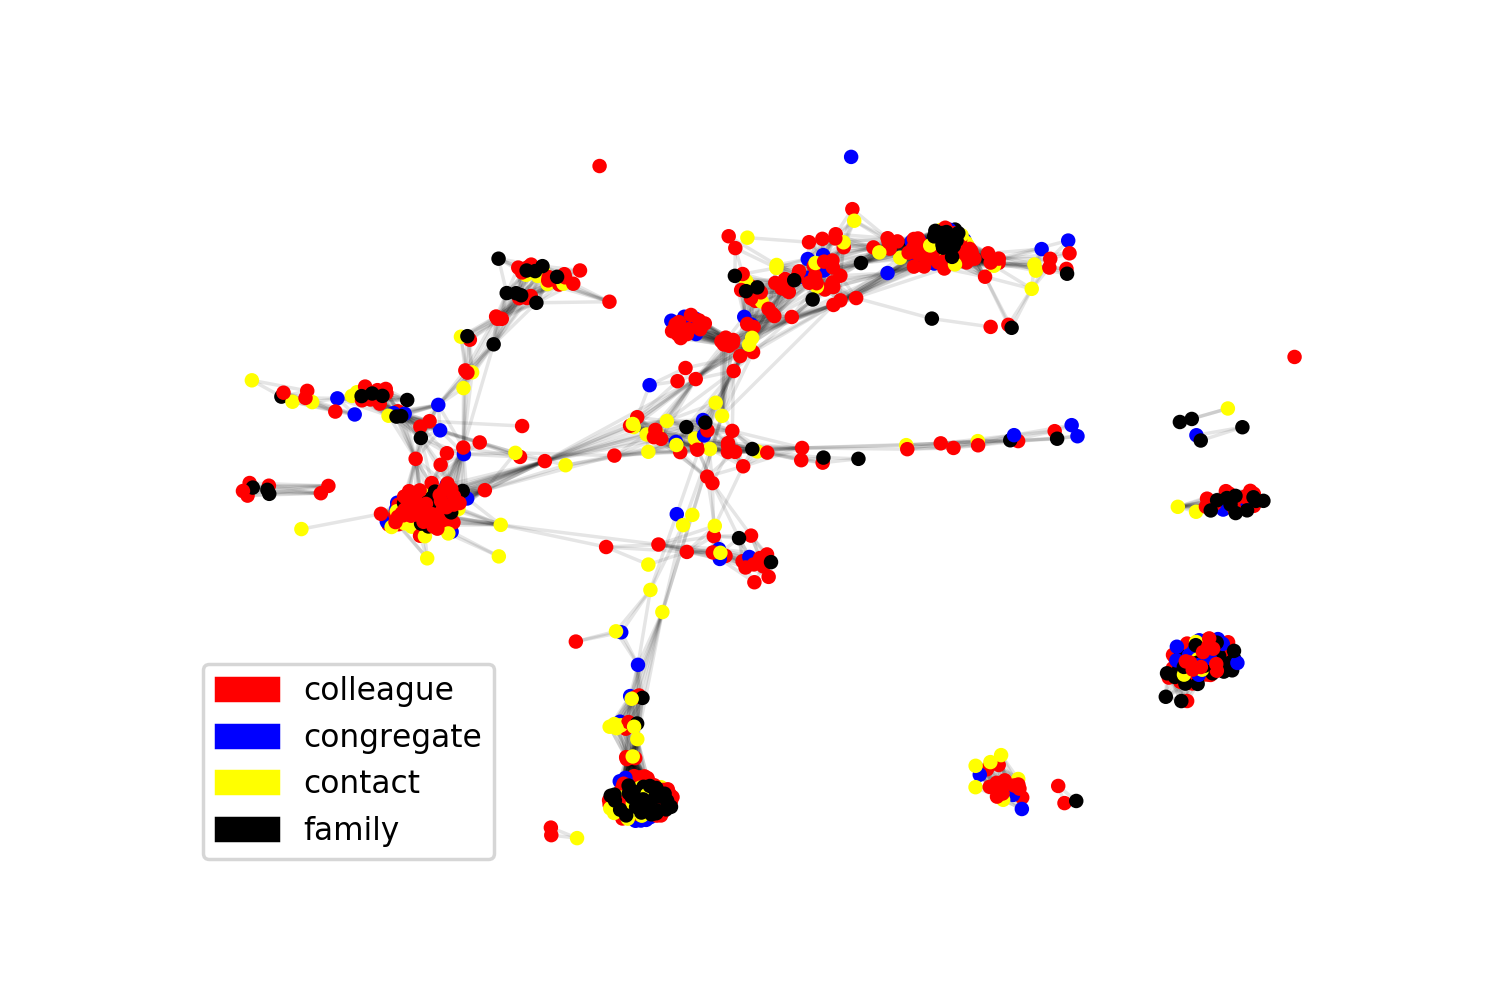
\includegraphics[width=.7\textwidth]{graphRel.png}
        \label{fig:graphLoc}
        \caption{Relationships dataset graph. The colouring of each node is related to its type of relation.}
        
\end{center}
\end{figure}

The relationships dataset represents the line graph of a network of relationships between terrorists. Each node represents a relationship between two terrorists. Two nodes are connected if they share a common terrorist. % and each edge a terrorist common to both connections. 
The label of each node relates to the nature of the relation between the two terrorists. It is an element of \{family, congregate, colleague, contact\}.

%\subsection{Terror Attacks Dataset}
%\label{subsec:Terror Attacks Dataset}

The terror attacks graph is built by connecting two nodes (terror attacks) if they share a common location. An other graph can be built by also connecting two terror attacks if they are perpetrated by the same organisation. This graph is not studied here.

\begin{figure}[t]
\begin{center}
    \begin{subfigure}[b]{0.45\textwidth}
        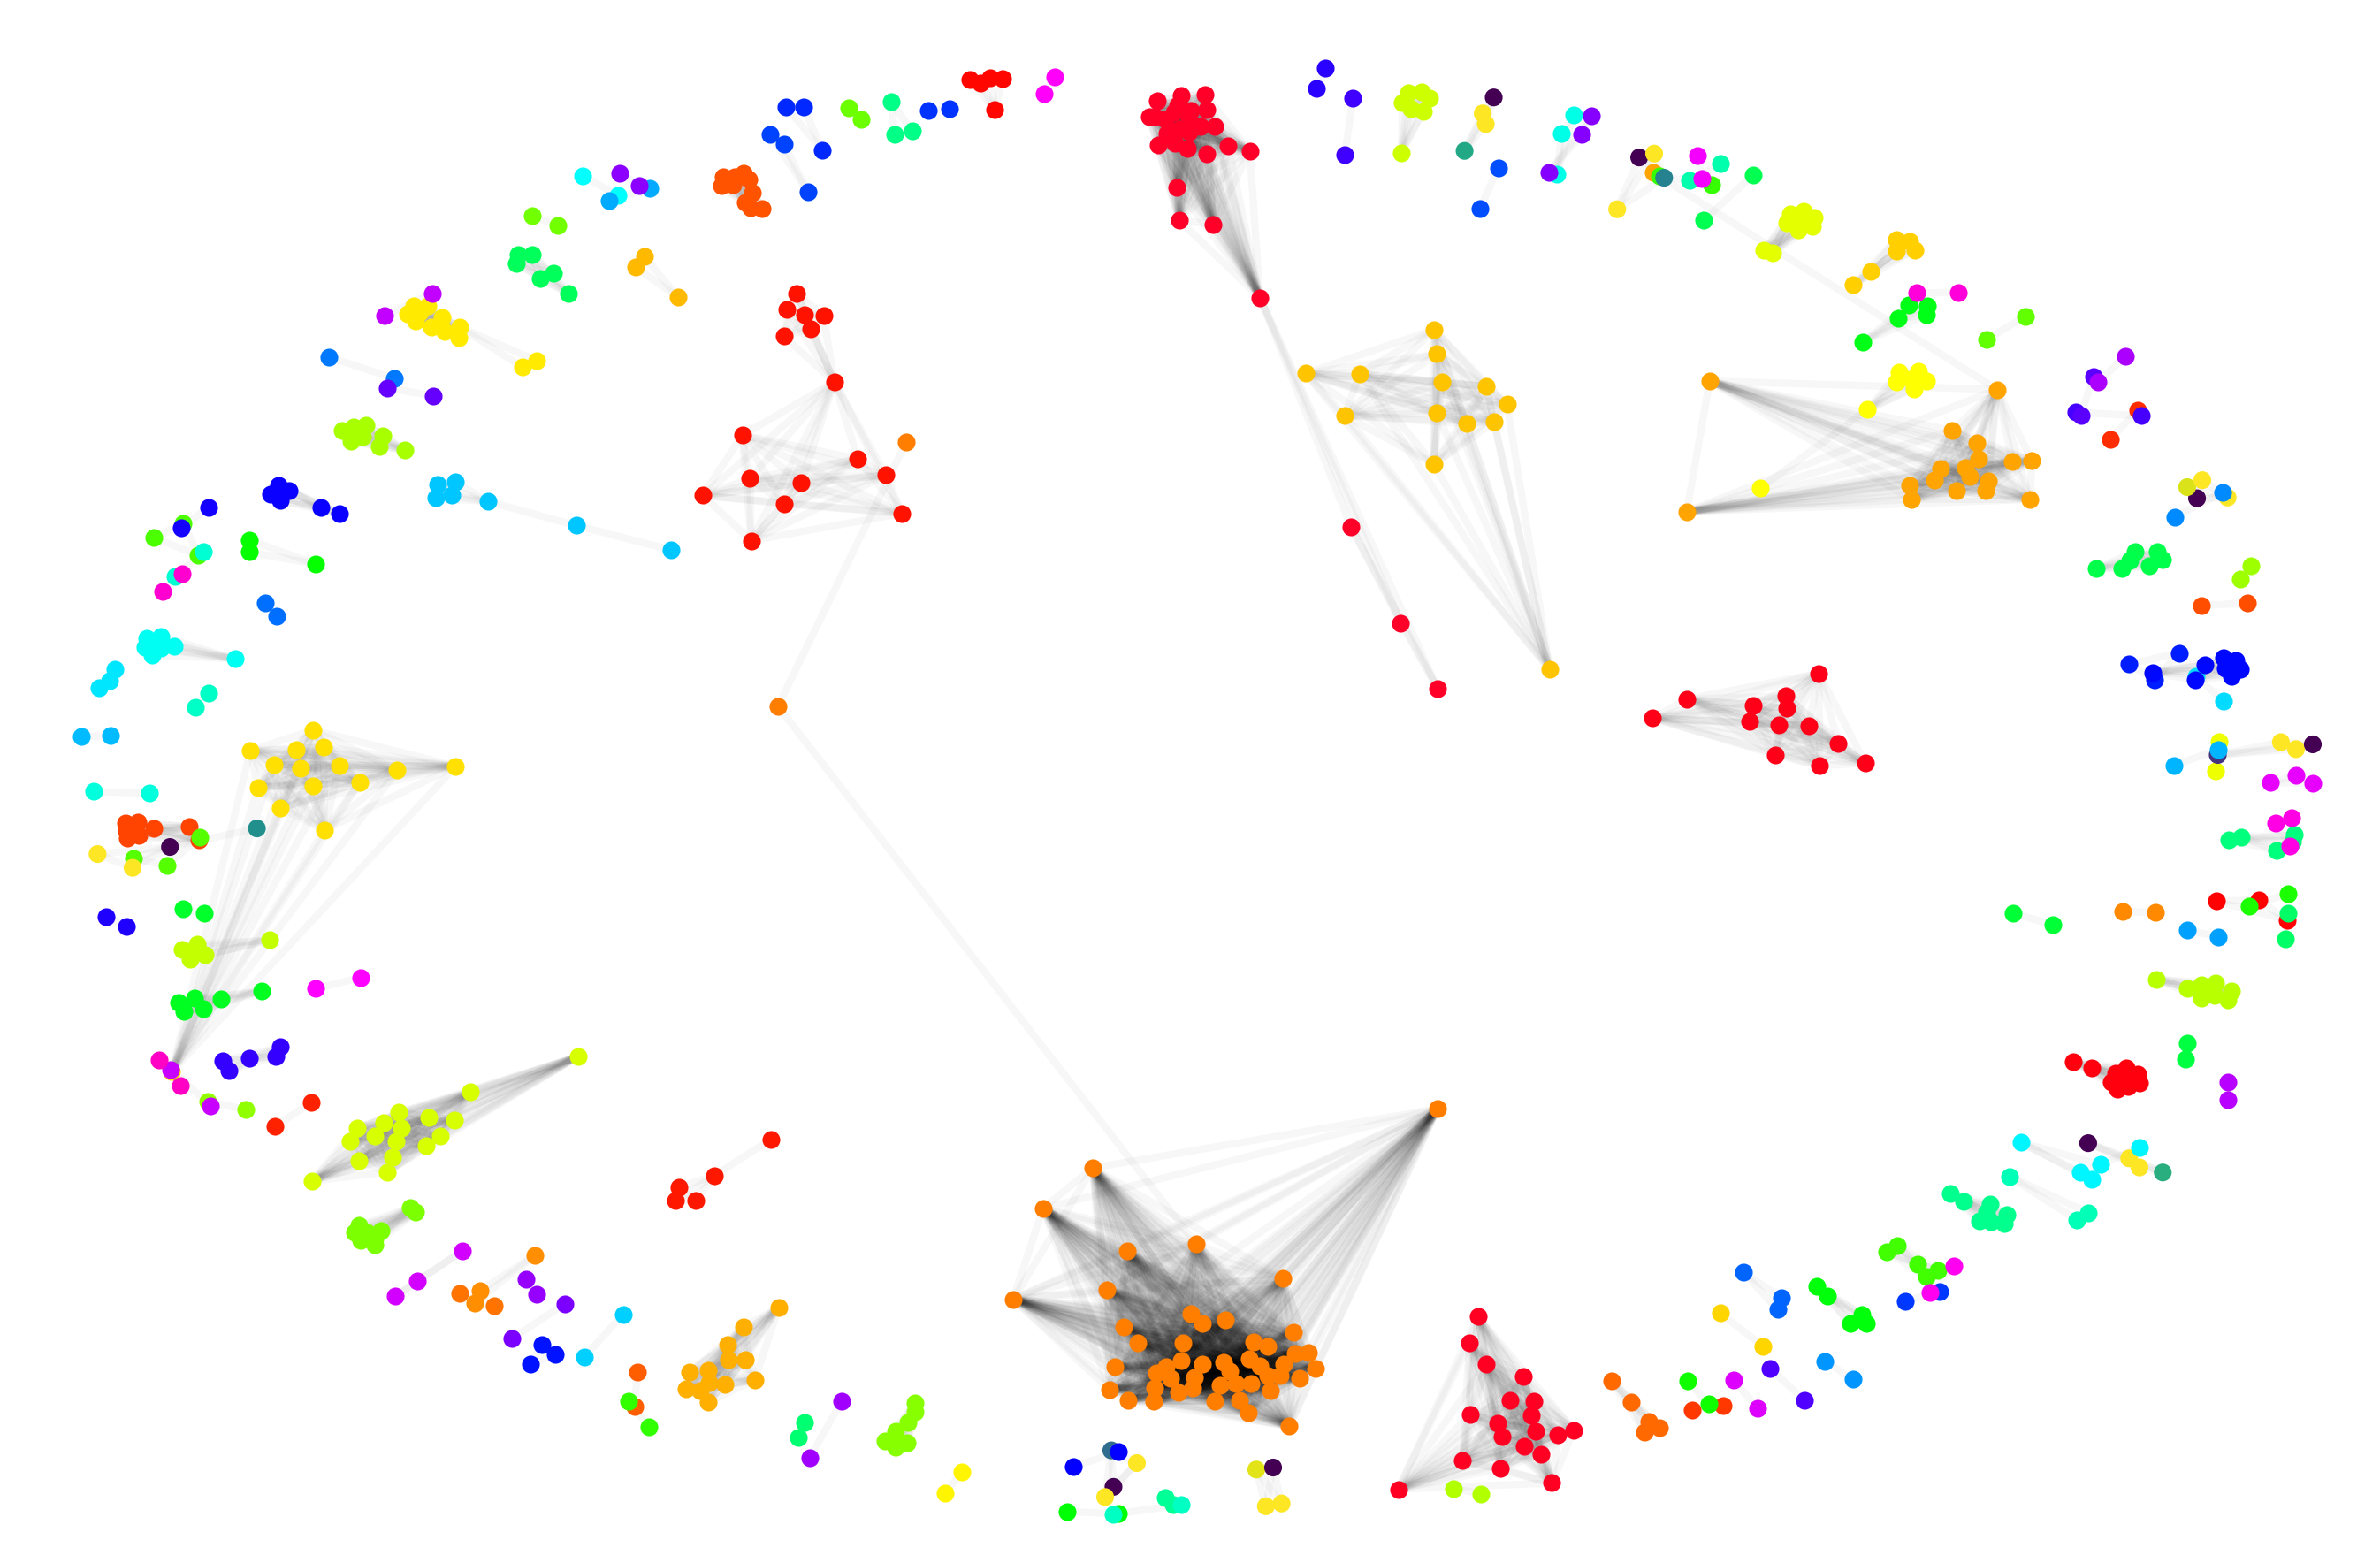
\includegraphics[width=\textwidth]{graphLoc.png}
        \caption{Terror attacks location graph, colouring by component ID}
        \label{fig:graphLoc}
    \end{subfigure}
    ~
    \begin{subfigure}[b]{0.45\textwidth}
        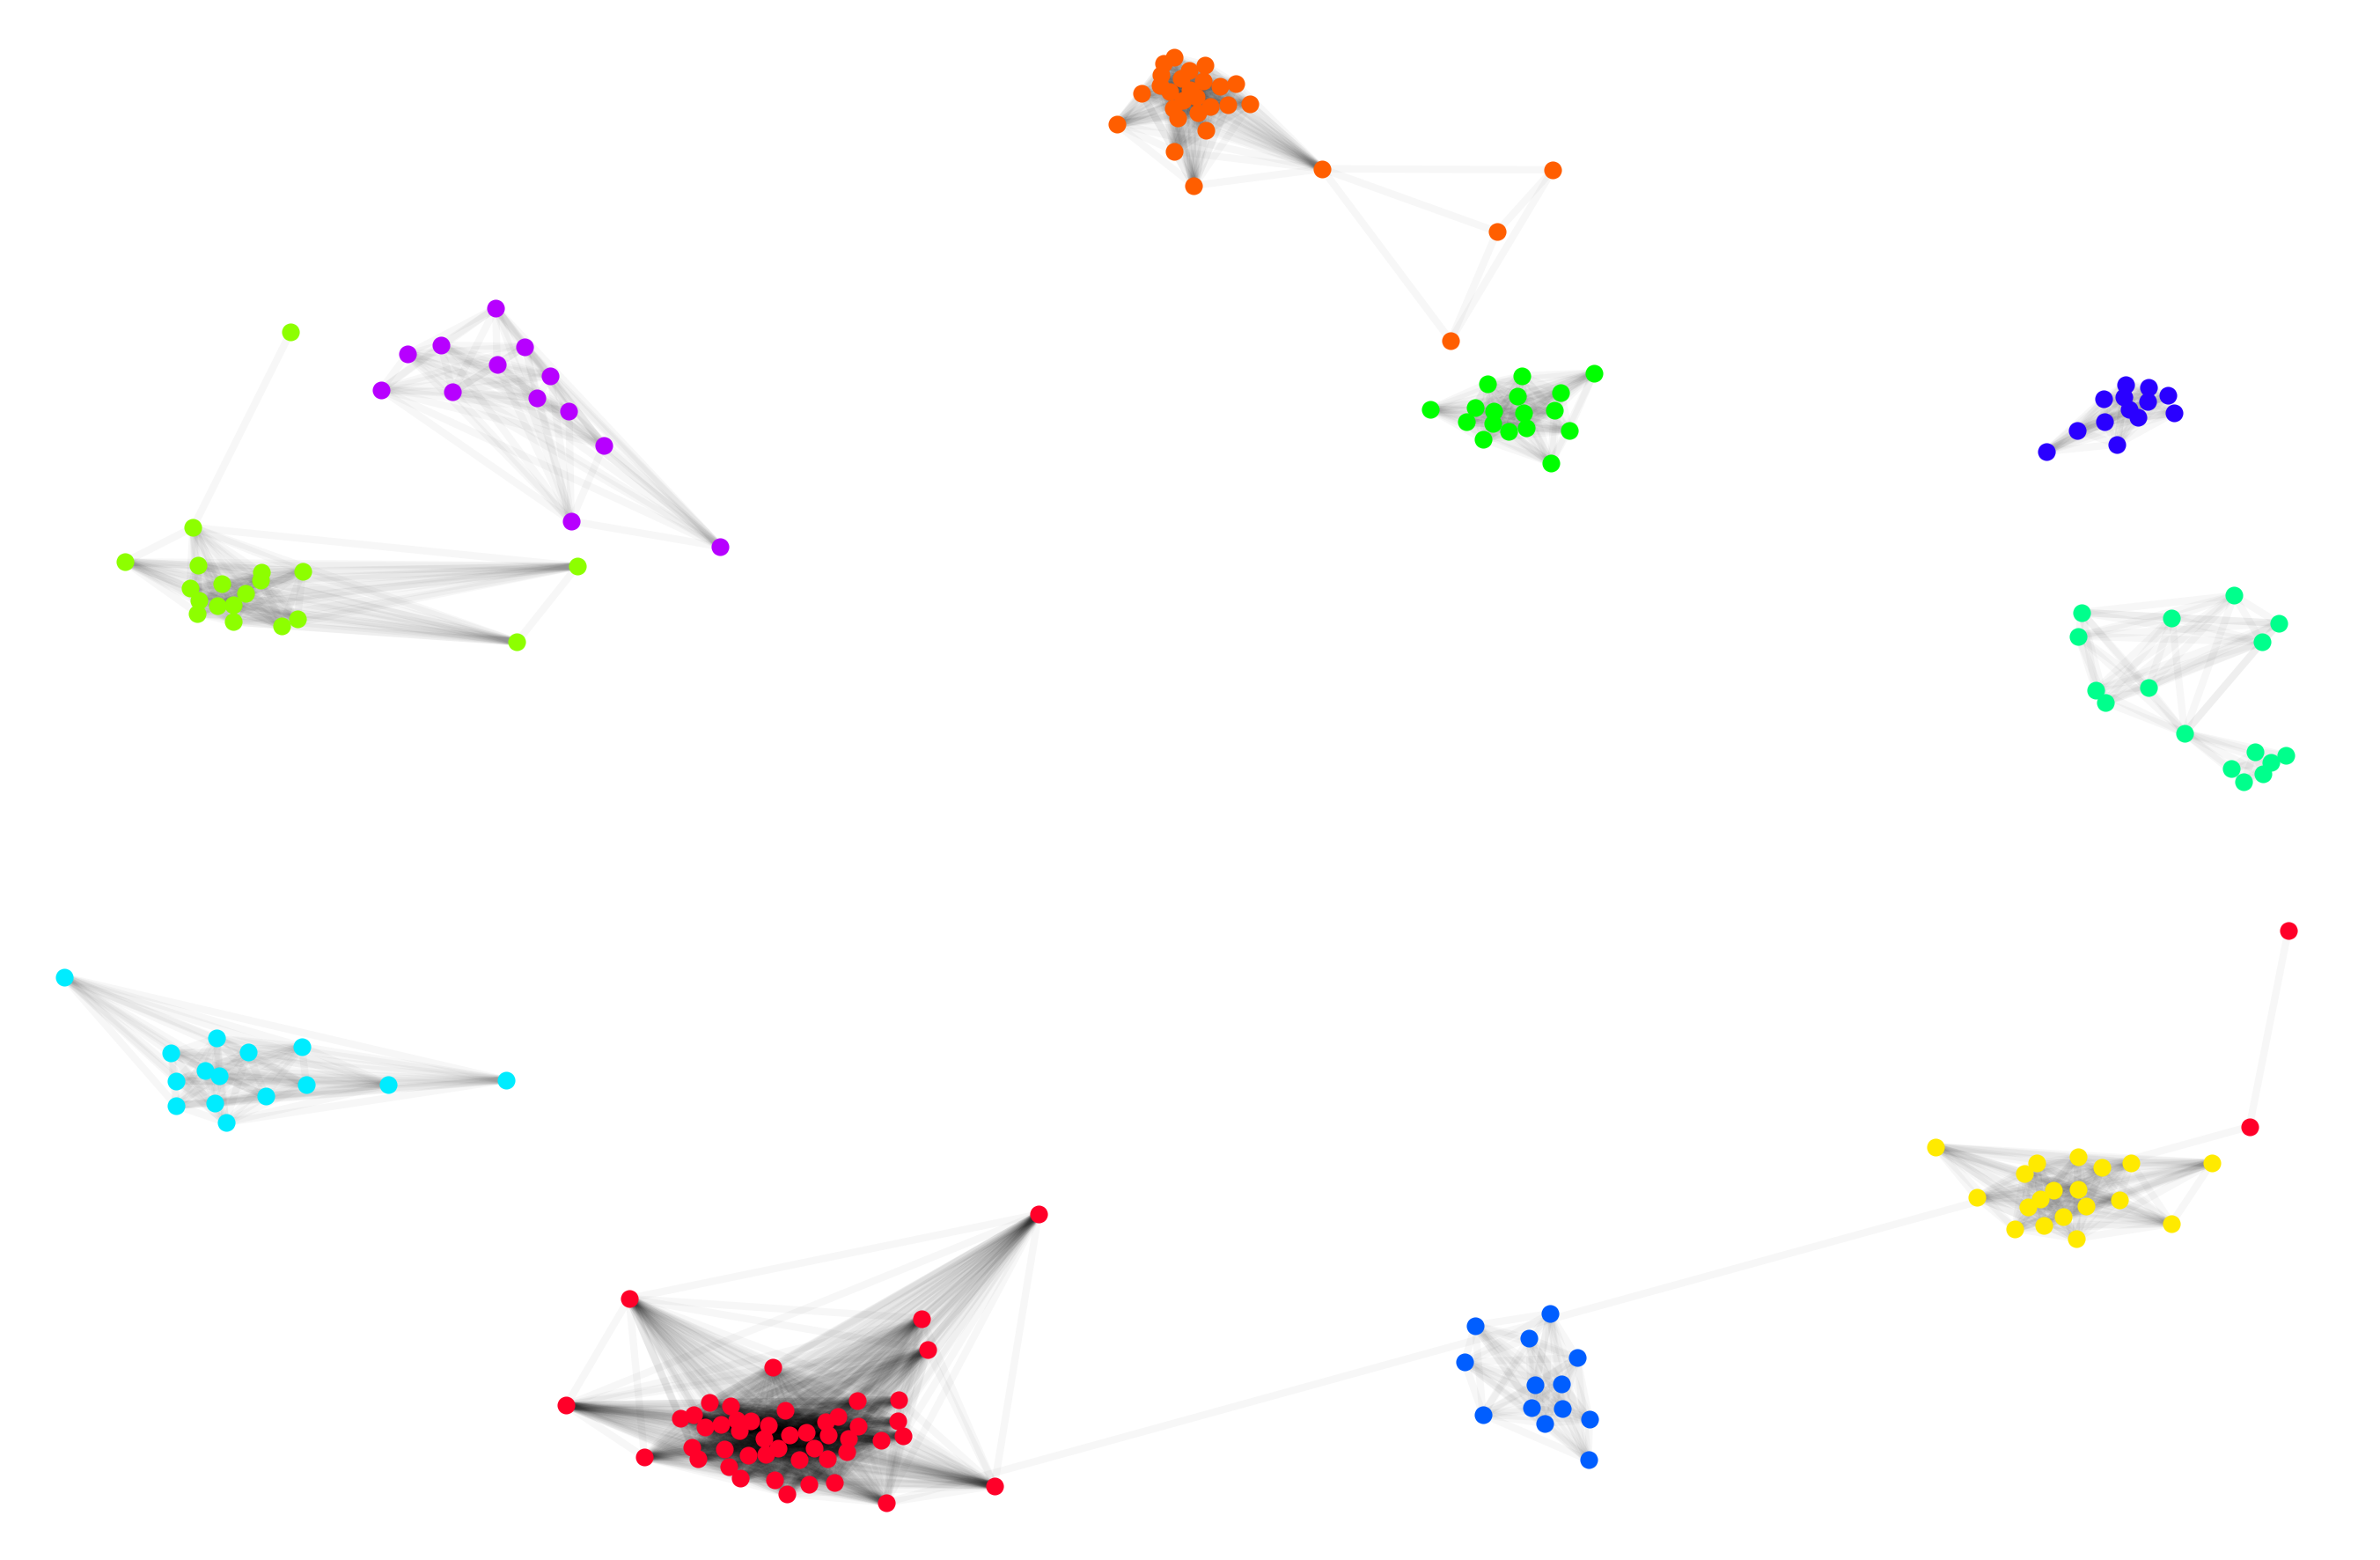
\includegraphics[width=\textwidth]{subGraph.png}
        \caption{Ten biggest components from the terror attacks location graph}
        \label{fig:subGraph}
    \end{subfigure}
\caption{Graphs from the terror attacks dataset}
\label{fig:graphPlots}
\end{center}
\end{figure}

Multiple issues have been found in this dataset:

\paragraph{Broadness} 
The dataset comprises attacks ranging from 1969 to 2005 and spanning the entire globe. Simple and relevant explanations for the graph formation or properties are not likely to be found, since the mechanisms behind two different attacks can be entirely different.

\paragraph{Structure} 
\label{par:Structure}
Half of the nodes are isolated, hence the topological information they carry in the graph is very limited. What is more, the construction of the graph implies a transitive relation inside connected components. Indeed, let $a$, $b$ and $c$ be terror attacks from the same connected component. Let ``$a\sim b$'' mean that terror attacks $a$ and $b$ took place close to each other. Then
\begin{equation}
\text{If } \left ( a \sim b \text{ and } b \sim c \right )  \text{ then probably } a \sim c
\label{eq:transitivity}
\end{equation}
This property translates into connected component that are almost complete -- hence bearing little topological information.

\paragraph{Reliability} 
As expected, errors have been found in the data. For example nodes
 \texttt{Djibouti\_Youth\_Movement\_19900927} 
 and 
 \texttt{Armed\_Islamic\_Group\_19950711} 
 have been connected, whereas the first attack took place in Djibouti~\cite{amnesty1991} and the second one in Paris~\cite{nouvelObs2007}. Hence algorithms using the data must tolerate some error in order to avoid overfitting.

\paragraph{Incompleteness}
The dataset has been constructed from publicly available sources~\cite{ZSG2006}. Because of the sensitivity of the data behind terrorist attacks and relationships, some of it is classified, making the dataset incomplete.

Further properties of the graphs are discussed below.

%Similarly to relationships datasets, we have found that the terrorist attacks dataset have very highly connected components, implying transitivity. 
%If attack $a$ took place close to $b$, and attack $b$ took place close to $c$, then it is probable that attack $a$ took place close to $c$.



\section{Terrorist Relationships as a Social Network}
\label{sec:Terrorist Relationships as a Social Network}
In this section, the properties of the terrorist relationships line graph as a relational network is explored. As~\cite{ZSG2006} mentions, an organisation needs interpersonal connection to function and studying the structure of the social organisation could allow to predict the evolution of terrorist organisations.

\cite{krawczyk_line_2011}~found that on the basis of a study of an online social network, such a network could be well approximated by the line graph of a scale free network. Assuming that there exists a transitivity relation between nodes (see Equation~\ref{eq:transitivity}) as one would expect in a social network, a scale free network corresponding to the relationships graph has been generated. Its line graph counterpart has then been compared to the relationships graph (see Figure~\ref{fig:RelationshipScaleFree} below).
%If that propriety can be verified by our dataset, %then we could gain information from the original graph from which the line graph originates.
%
%Social sciences studies have shown that social/relationship networks have the particularities of homophily and transitivity.
%Logically if $a$ \& $b$ are friends and $c$\& $b$ are also, the it is more likely that $a$ \& $c$ are friends than not. This mathematically translates to:
%\begin{equation}
%	a \sim b \text{ and } b \sim c \text{ then } a \sim c
%\end{equation}
%
%As a first research question we will try to verify that our dataset derives from a scale-free network, implying that the graph that generated the relationship dataset have proprieties similar to social networks.
%By creating a scale-free network and making its line graph, we compared the degree distribution of the relationship dataset we were able to show that.

\begin{figure}[H]
\begin{center}
    \begin{subfigure}[b]{0.4\textwidth}
        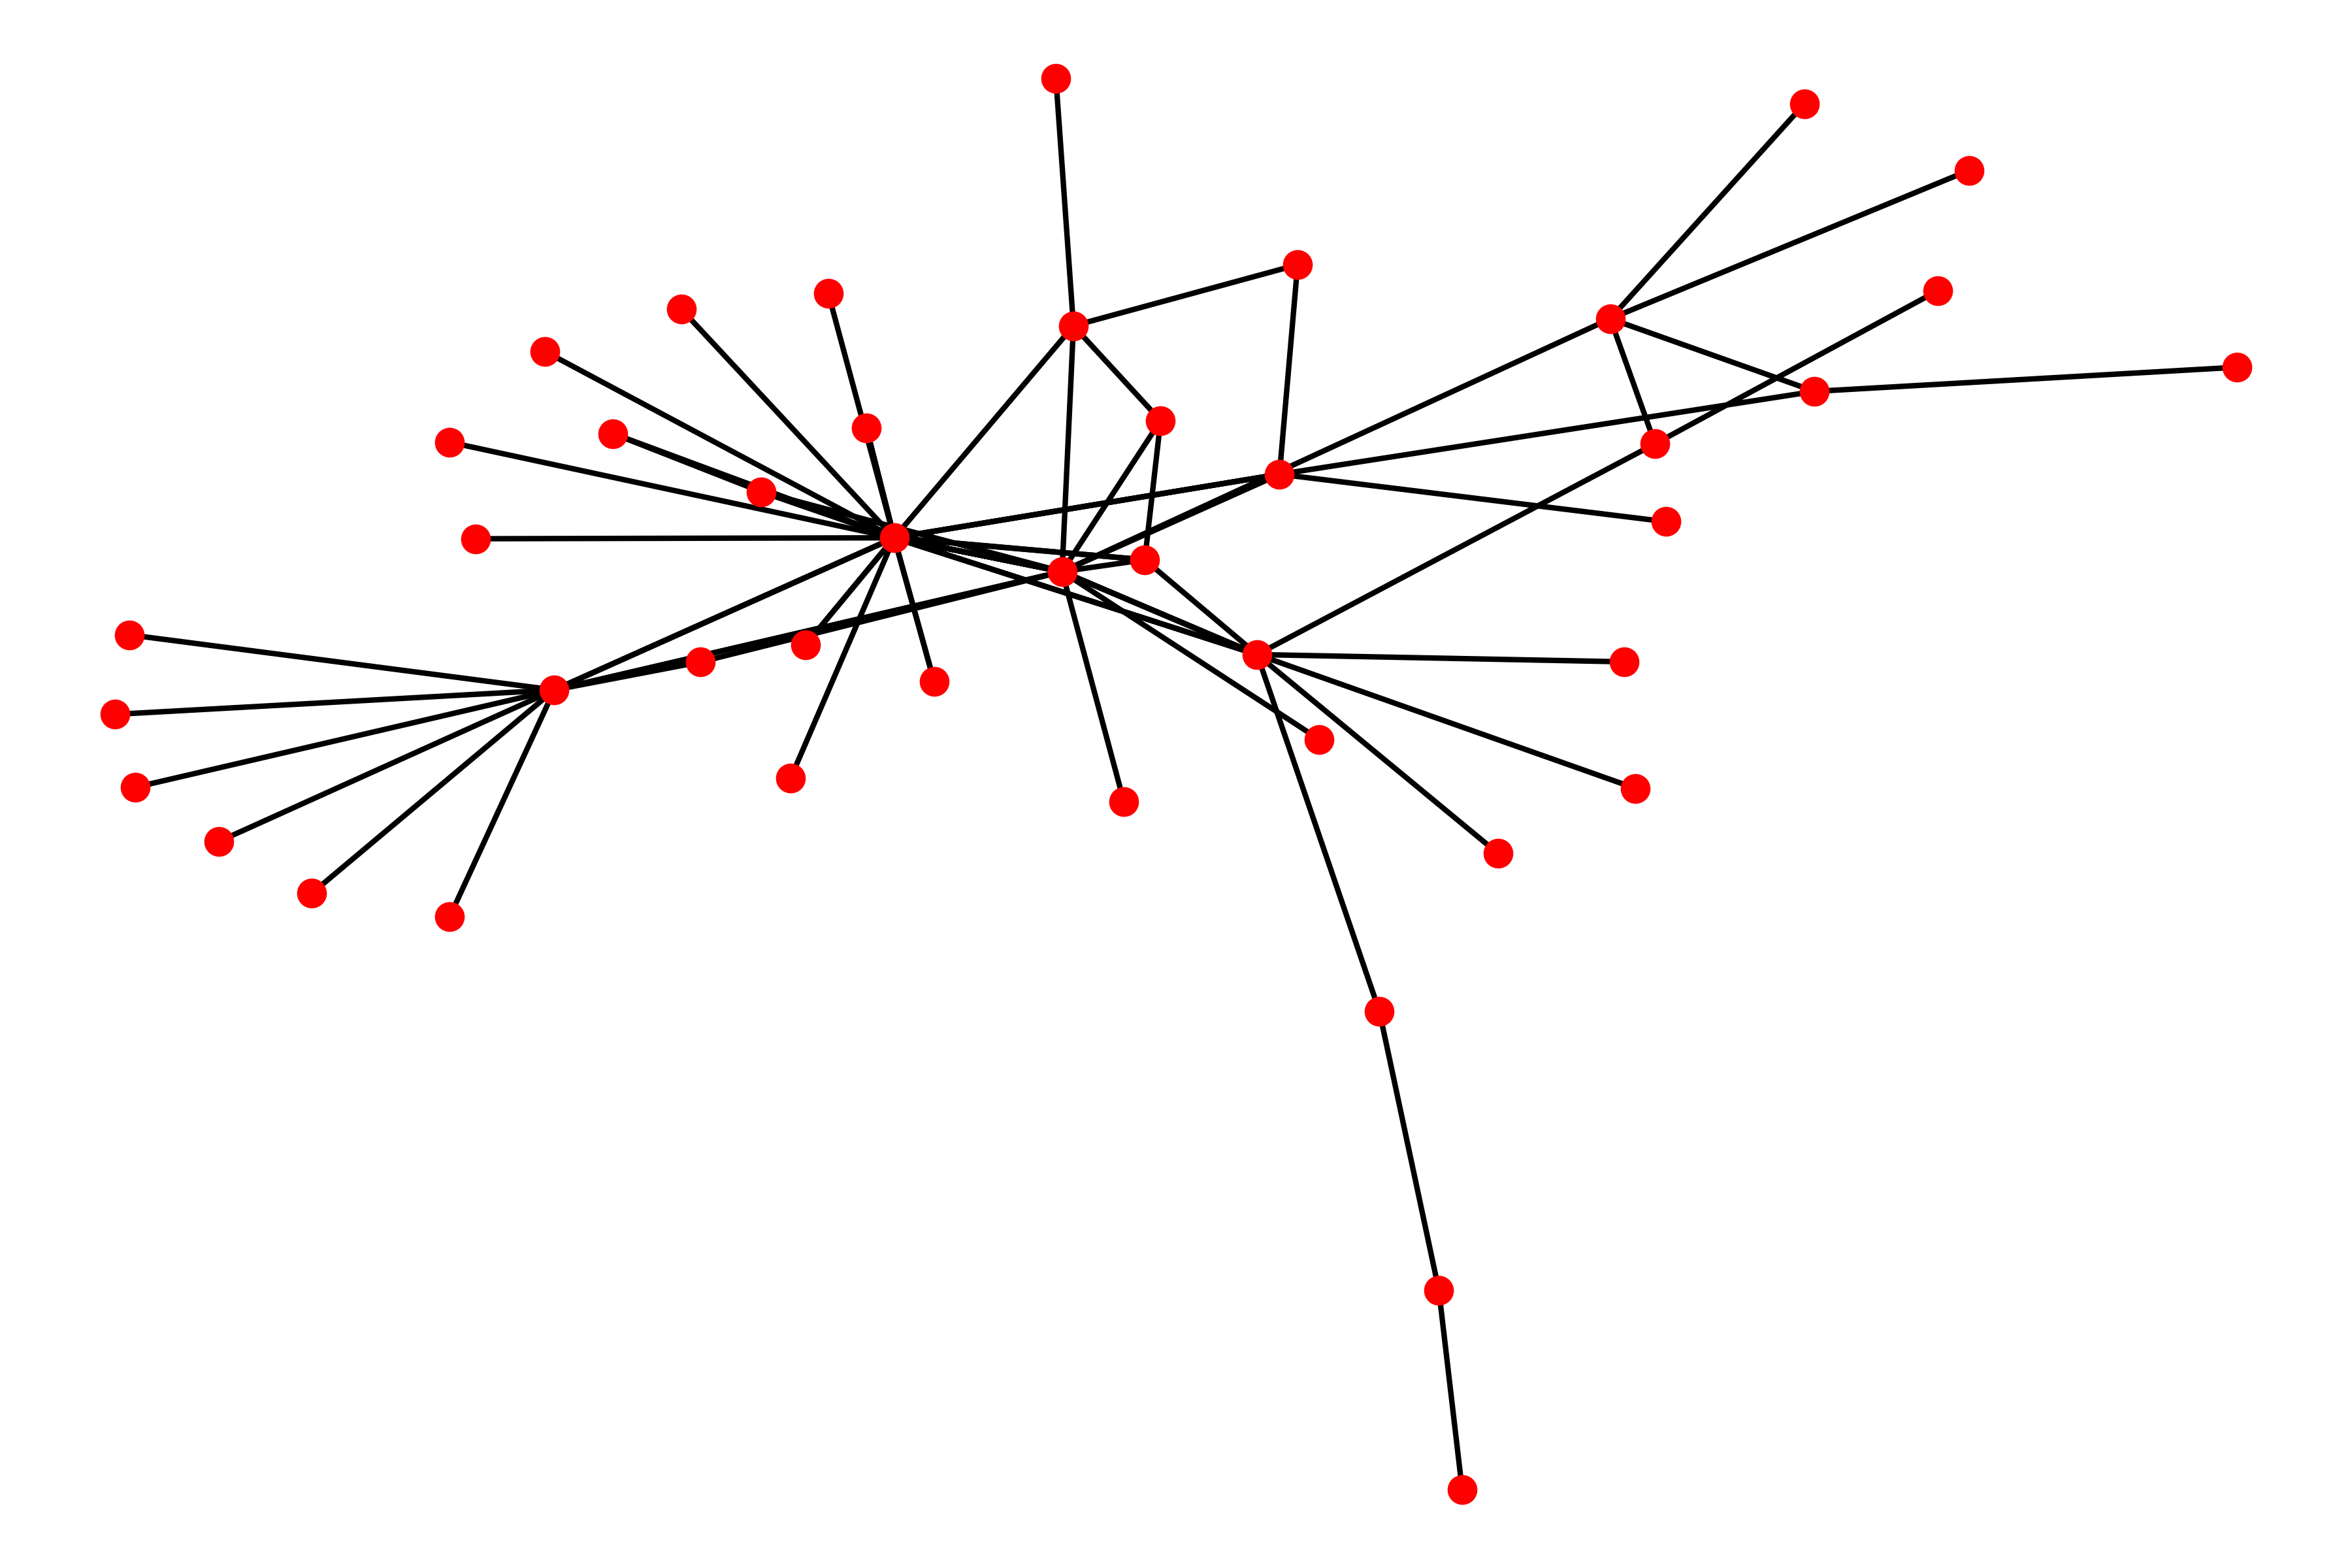
\includegraphics[width=\textwidth]{graphScaleFree.png}
        \caption{Scale free network}
        \label{fig:Scalefree}
    \end{subfigure}
    ~
    \begin{subfigure}[b]{0.4\textwidth}
        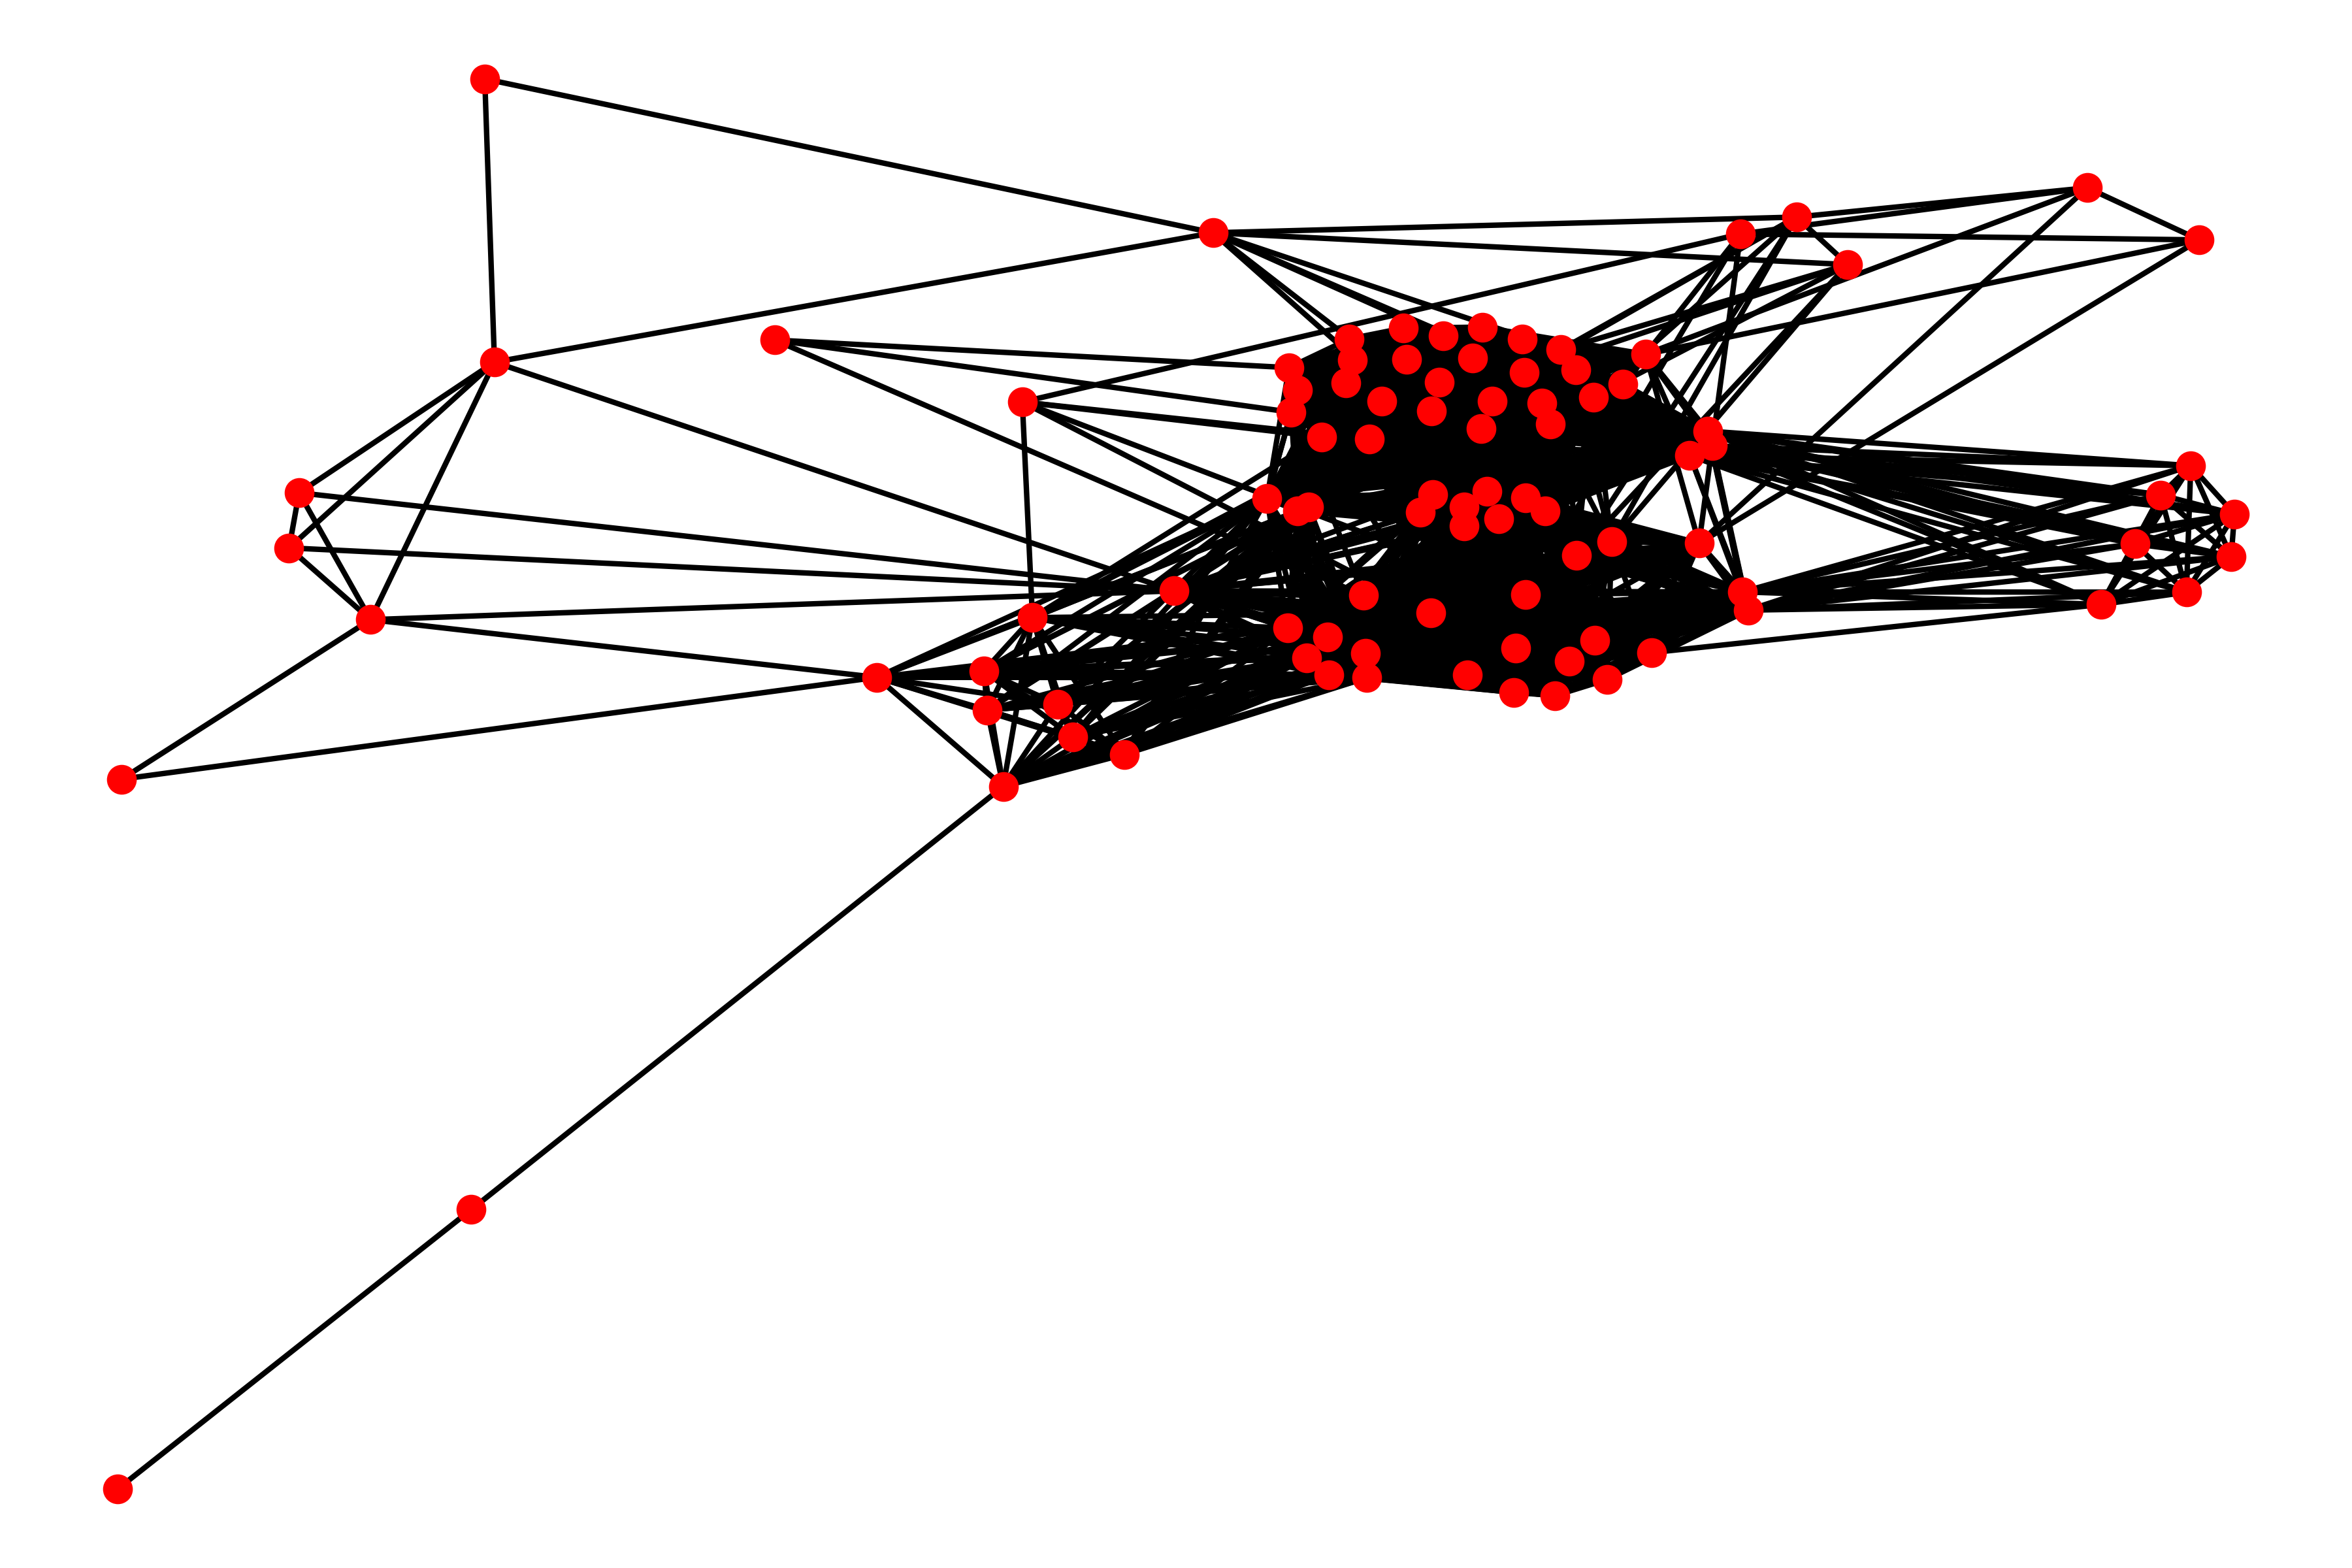
\includegraphics[width=\textwidth]{graphLineScaleFree.png}
        \caption{Line graph of scale free network}
        \label{fig:lineG}
    \end{subfigure}
    
    \begin{subfigure}[b]{\textwidth}
    	\begin{centering}
        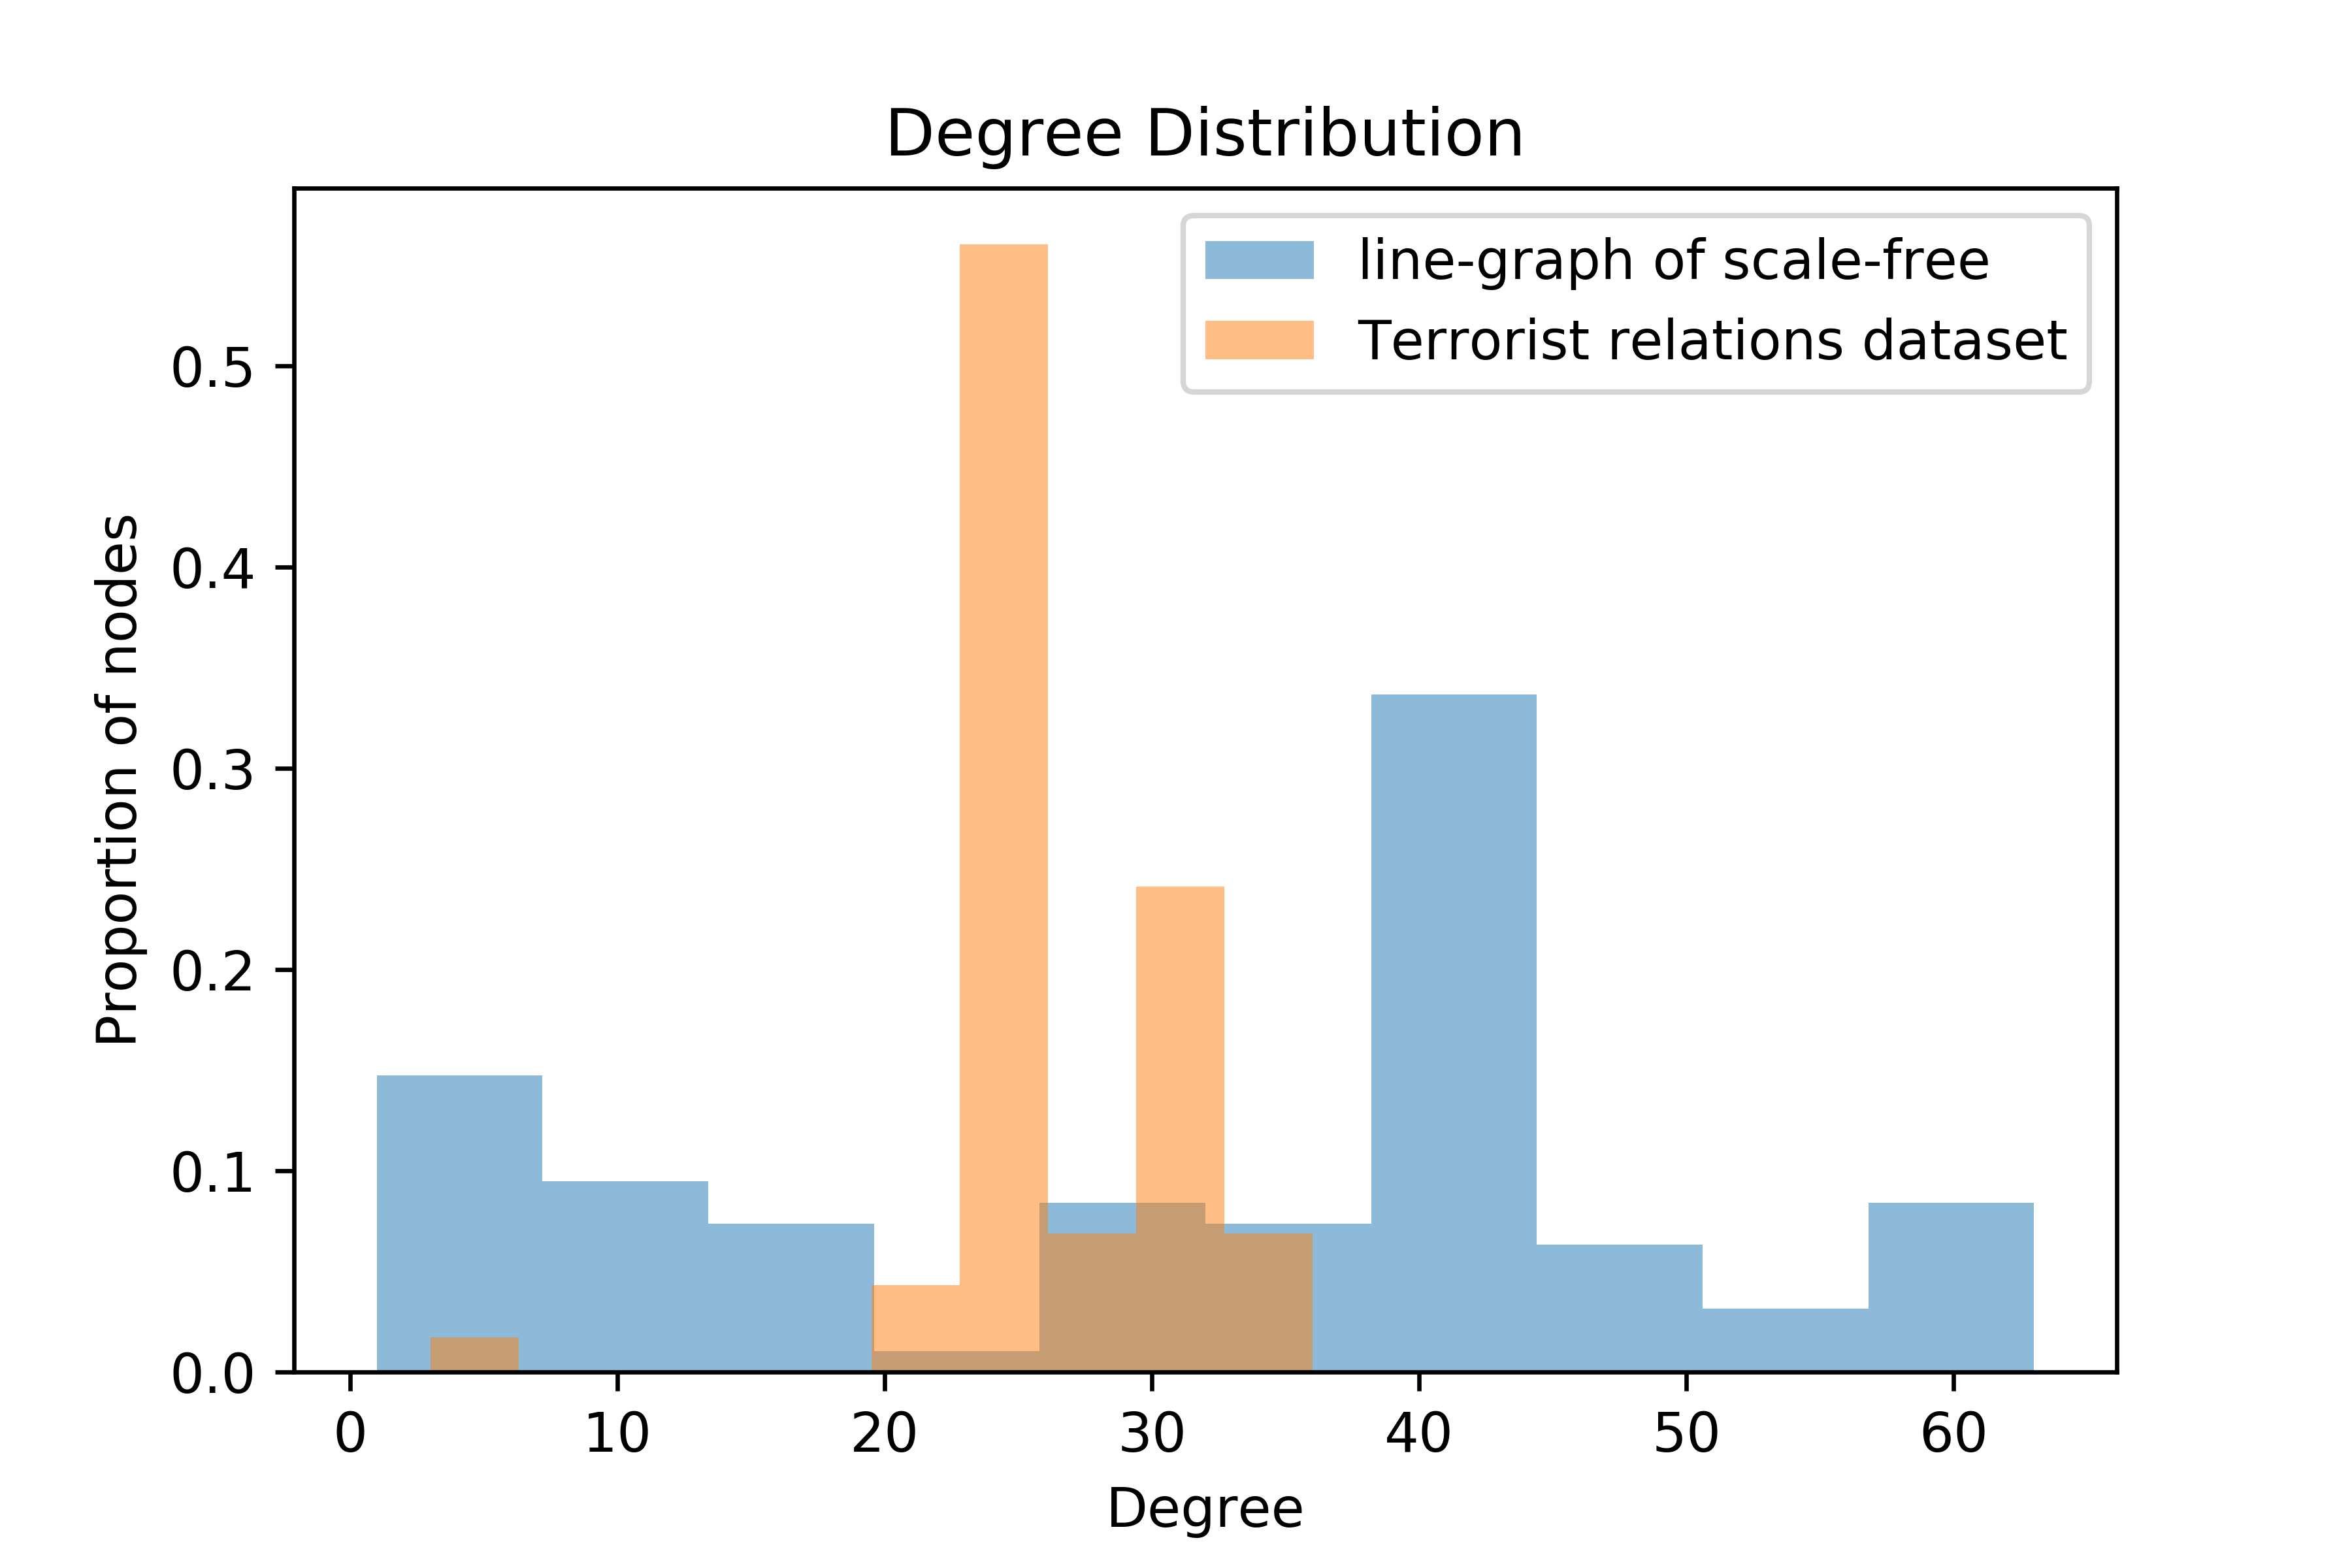
\includegraphics[width=.5\textwidth]{DegreeDiff.png}
        \caption{\centering Comparison of the degree distribution of the two line graphs.}
        \label{fig:DegDiff}
        \end{centering}
    \end{subfigure}
\caption{Comparison of a scale free network and the terrorist relationships network.}
\label{fig:RelationshipScaleFree}
\end{center}
\end{figure}

From the degree distribution comparison, we can conclude that the terrorist relationships network shows no significant similarity with a  social network. 
%\subsection{Terrorist Relations Dataset}
%
%\subsection{Terror Attacks Dataset}
%\label{subsec:terror attack quality}


\section{Predictions}
\label{sec:Predictions}

The algorithm used to predict the terror attack location is the following:

L

\begin{table}[H]
\caption{Prediction accuracy for different node distance weightings}
\begin{center}
\begin{tabular}{l l l l}
\multicolumn{2}{l}{
\textbf{Weighting}}														& \textbf{Best skewness $\zeta$}		& \textbf{Accuracy}\\

Gaussian:			& $w=e^{-d^2/\zeta}-e^{-1/\zeta}$							& \SI{0.01}{}						&\SI{50.5}{\percent} \\

Log-Exponential:	& $w=e^{-d} \log\left( \frac{1+\zeta}{d+\zeta}\right)$				&\SI{0.1}{}							& \SI{50}{\percent} \\ 

Linear:			& $w=1-d$											& N.A. 							&\SI{47}{\percent} \\

Square:			&$w= \begin{cases}
1				&d < \zeta \\
0				& \text{otherwise}
				\end{cases}$											& \SI{0.1}{}						& \SI{43}{\percent}
\end{tabular}
\end{center}
\label{default}
\end{table}

\section{Conclusion}
\label{sec:Conclusion}
Section~\ref{subsec:terror attack quality} explains that the ``Terror Attacks" dataset contains flaws that make it difficult to analyze.

However, the results in Table~\ref{tab:results} show that predicting the location of an attack with its features is feasible even though the prediction is not very efficient. This result suggests that there is a link between the location of an attack and its characteristics (such as the type of the attack).

\bibliographystyle{ieeetr}
\bibliography{bib}

\end{document}  